\def\pgfsysdriver{pgfsys-dvisvgm.def}
\documentclass[dvisvgm,tikz,border=10pt]{standalone}
\usepackage{tikz}
\usepackage{amsmath}
\usetikzlibrary{arrows.meta,patterns,positioning}
\tikzset{
 clause/.style={rectangle,draw=black,fill=white,minimum size=7mm,line width=.9pt},
 varnode/.style={circle,draw=black,minimum size=9mm,line width=.9pt},
 truevar/.style={varnode,fill=white},
 falsevar/.style={varnode,fill=gray!55},
 freevar/.style={varnode,pattern=north east lines,pattern color=gray!65},
 positive/.style={draw=black,line width=1pt},
 negative/.style={positive,dash pattern=on 4pt off 3pt},
 every node/.style={text=black,font=\sffamily},
}

\begin{document}
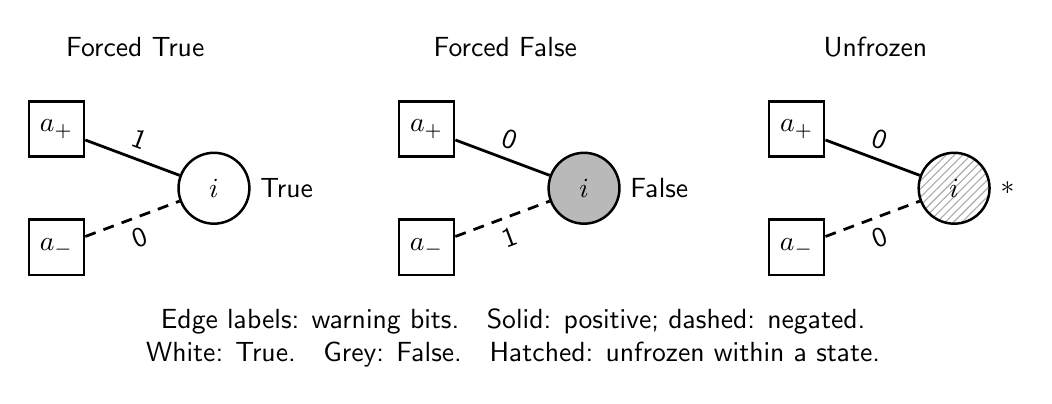
\begin{tikzpicture}
\begin{scope}
\node at (1,1.8) {Forced True};
\node[clause] (p1) at (0,.75) {$a_+$};
\node[clause] (n1) at (0,-.75) {$a_-$};
\node[truevar,label=right:True] (i1) at (2,0) {$i$};
\draw[positive] (p1)--node[above,sloped] {1} (i1);
\draw[negative] (n1)--node[below,sloped] {0} (i1);
\end{scope}
\begin{scope}[xshift=4.7cm]
\node at (1,1.8) {Forced False};
\node[clause] (p2) at (0,.75) {$a_+$};
\node[clause] (n2) at (0,-.75) {$a_-$};
\node[falsevar,label=right:False] (i2) at (2,0) {$i$};
\draw[positive] (p2)--node[above,sloped] {0} (i2);
\draw[negative] (n2)--node[below,sloped] {1} (i2);
\end{scope}
\begin{scope}[xshift=9.4cm]
\node at (1,1.8) {Unfrozen};
\node[clause] (p3) at (0,.75) {$a_+$};
\node[clause] (n3) at (0,-.75) {$a_-$};
\node[freevar,label=right:{$\ast$}] (i3) at (2,0) {$i$};
\draw[positive] (p3)--node[above,sloped] {0} (i3);
\draw[negative] (n3)--node[below,sloped] {0} (i3);
\end{scope}
\node[align=center] at (5.8,-1.9) {Edge labels: warning bits.\quad
Solid: positive; dashed: negated.\\
White: True.\quad Grey: False.\quad Hatched: unfrozen within a state.};
\end{tikzpicture}
\end{document}
